% 浙江大学《海洋大数据技术原理与应用》课程论文。编译：bash build.sh
\documentclass[zihao=5, a4paper, oneside]{ctexart}

% ---------- 版面 ----------
\usepackage[top=2.54cm, bottom=2.54cm, left=3.0cm, right=2.6cm, headheight=15pt]{geometry}
\usepackage{setspace}
\setstretch{1.3}
\setmainfont{Times New Roman}
\setCJKmainfont[BoldFont=SimHei, ItalicFont=KaiTi]{SimSun}
\setCJKsansfont{SimHei}
\setCJKfamilyfont{hei}{SimHei}
\setCJKfamilyfont{kai}{KaiTi}
\usepackage{amsmath, amssymb, bm}
\usepackage{graphicx, subcaption, booktabs, multirow, array}
\usepackage[table]{xcolor}
\usepackage{algorithm}
\usepackage{algpseudocode}
\usepackage[hidelinks]{hyperref}
\usepackage{fancyhdr}
\usepackage[sort&compress, square, comma, numbers]{natbib}
\renewcommand{\bibfont}{\small}
\setlength{\bibsep}{1.5pt}
\usepackage{caption}
% floats never cross into the next section; at most one float at the top of a page,
% so figures alternate with the text that discusses them
\usepackage[section]{placeins}
\setcounter{topnumber}{2}
\setcounter{bottomnumber}{1}
\setcounter{totalnumber}{3}
\renewcommand{\topfraction}{0.8}
\renewcommand{\bottomfraction}{0.62}
\renewcommand{\textfraction}{0.15}
\renewcommand{\floatpagefraction}{0.7}

\captionsetup{font=small, labelsep=quad, labelfont=bf}
\captionsetup[figure]{name=图}
\captionsetup[table]{name=表}
\floatname{algorithm}{算法}
\renewcommand{\algorithmicrequire}{\textbf{输入：}}
\renewcommand{\algorithmicensure}{\textbf{输出：}}
\graphicspath{{figures/}}

% 标题样式：1 绪论 / 1.1 研究背景 / 1.1.1
% a float defined under a heading never goes to the top of the page above that heading
\ctexset{
  section = {format=\zihao{4}\heiti, beforeskip=14pt, afterskip=8pt, name={,}, number=\arabic{section},
             aftertitle=\suppressfloats[t]},
  subsection = {format=\zihao{-4}\heiti, beforeskip=10pt, afterskip=5pt, aftertitle=\suppressfloats[t]},
  subsubsection = {format=\zihao{5}\heiti, beforeskip=6pt, afterskip=3pt},
}

% 页眉页脚
\pagestyle{fancy}
\fancyhf{}
\fancyhead[C]{\zihao{5}\songti 海洋大数据技术原理与应用\quad 课程论文}
\fancyfoot[C]{\zihao{5}\thepage}
\renewcommand{\headrulewidth}{0.6pt}

\newcommand{\coverline}[2]{{\heiti\makebox[5.4em][s]{#1}}：\ \underline{\makebox[15em][c]{#2}}}
\newcommand{\TBD}[1]{\textcolor{red}{[待补：#1]}}

\begin{document}

% ---------- 封面（浙江大学课程论文样式：校名题字、课程名、校徽、信息栏） ----------
\begin{titlepage}
  \centering
  \singlespacing
  \vspace*{0.6cm}
  
\includegraphics[width=0.40\textwidth]{logo/zjuchar}\par
  \vspace{0.8cm}
  {\zihao{-1}\heiti 《海洋大数据技术原理与应用》课程论文\par}
  \vspace{1.0cm}
  
\includegraphics[width=0.27\textwidth]{logo/zju}\par
  \vspace{1.0cm}
  {\zihao{-2}\heiti 合理反例检验：粗分辨率海流图下自主水下航行器何时计算、何时观测
\par}
  \vspace{1.1cm}
  {\zihao{4}
  \begin{tabular}{@{}l@{}}
    \coverline{学年学期}{2026--2027 学年秋学期}\\[10pt]
    \coverline{姓名与学号}{徐陈栋\quad 3240100538}\\[10pt]
    \coverline{年级与专业}{24 级海洋工程与技术}\\[10pt]
    \coverline{任课教师}{张帆\quad 研究员}\\[10pt]
    \coverline{开课学院}{海洋学院}
  \end{tabular}\par}
  \vspace{0.9cm}
  {\zihao{5}\heiti 代码、数据与人机对话记录\par}
  \vspace{2pt}
  {\zihao{5}\url{https://github.com/frankxucd0826-source/auv-compute-or-observe}\par}
  \vfill
  {\zihao{4}\heiti 2026 年 11 月\par}
  \vspace{0.8cm}
\end{titlepage}

% ---------- 题目、作者与摘要（期刊论文版式） ----------
\pagenumbering{arabic}
\begin{center}
  {\zihao{-2}\heiti 合理反例检验：粗分辨率海流图下自主水下航行器何时计算、何时观测
\par}
  \vspace{6pt}
  {\zihao{4}\kaishu 徐陈栋\par}
  {\zihao{5}\songti （浙江大学\ 海洋学院，浙江\ 舟山\ 316021）\par}
\end{center}
\vspace{4pt}
{\heiti 摘要：}
自主水下航行器（下称航行器）已能在强流海区执行长航程任务，其航路规划依赖岸基系统发布的海流图。受水声通信带宽与上浮代价的限制，航行器在航行中往往只有一张数天前的粗分辨率海流图（下称粗图）；绕越禁航区时，从左侧还是右侧通过是不可逆的选择，选错一侧要多花数小时。现有方法难以判断粗图能否支撑这一选择：加密求解网格只能减小求解误差，纠正不了粗图本身的误差；集合规划需要在大量随机流场上求解，且只统计改变选边的成员比例，不衡量选错的代价；自适应采样以降低全场的估计误差为目标，测量的未必是决定选边的海流。为此，本文提出合理反例检验：在与粗图相容的合理流场集合中，搜索使另一侧更快的流场（合理反例），以坚持当前选择最多多花的航时（最大后悔值）判断粗图是否可信，并据此决定继续计算还是获取新信息。该方法有三个要点：一是用多年再分析数据中粗图的误差，标定合理流场集合的误差大小、空间相关长度与半径；二是利用包络定理沿最快航线累加航时对流场的导数，约71次航线求解即可完成搜索；三是两侧航时差小于求解误差时才加密网格，最大后悔值超过阈值时上浮获取新的海流图，不能上浮时改选最大后悔值较小的一侧。我们在黑潮、湾流、阿古拉斯回流区以及改带卫星测高地转流图的黑潮区共2532个测试任务上，将该方法与加密求解、集合规划、就地测流和总是上浮等做法比较。结果表明，计算量增加64倍几乎不降低选错率，换用当天0.5°海流图则使之降至7\%--10\%；按最大后悔值排在前20\%的任务集中了全部额外航时（比真实更快一侧多花的航时）的53\%--71\%，高于按改变选边的成员比例排序的36\%--52\%；在黑潮，梯度搜索以约二十九分之一的求解次数达到集合平均选边的效果；在湾流与阿古拉斯回流区，对判定不可信的任务上浮取图，使平均额外航时分别从3.56小时降至1.31小时、从6.87小时降至2.20小时。这表明，粗图缺失的信息无法靠端侧计算补足，合理反例检验为航行器在计算与观测之间的取舍提供了可计算的判据。

{\heiti 关键词：}海洋大数据；自主水下航行器；航路规划；不确定性量化；最大后悔值；合理反例检验

\vspace{1em}
\begin{center}
{\large\bfseries Plausible Counterexample Test: When an Autonomous Underwater Vehicle Should Compute and When It Should Observe Under a Coarse Current Map}
\end{center}
\vspace{0.5em}

{\bfseries Abstract:}
Autonomous underwater vehicles (AUVs) now carry out long missions in strong-current regions, and their route planning relies on current maps issued by shore-based systems. Because acoustic links are slow and surfacing interrupts the mission, a vehicle at sea usually holds only a coarse current map issued days earlier. When it passes a no-go zone, the choice between the left and the right side cannot be undone, and the wrong side costs hours. Existing methods cannot tell whether the map supports this choice: a finer solver reduces numerical error but not the error of the map itself; ensemble planning needs many sampled currents and counts how many members change the side rather than what a wrong side costs; adaptive sampling reduces the error of the whole field instead of measuring the currents that decide the side. We propose a plausible counterexample test. It searches the set of currents consistent with the map for one that makes the other side faster (a plausible counterexample), uses the largest extra time of keeping the current choice (the maximum regret) to judge whether the map can be trusted, and on that basis decides whether to compute more or to acquire new information. The test has three parts. The set of plausible currents is calibrated from the errors of the map in multi-year reanalysis data. The derivative of travel time with respect to the current is accumulated along the fastest route by the envelope theorem, so the search needs about 71 route solves. A finer grid is used only when the two sides differ by less than the numerical error, and when the maximum regret exceeds a threshold the vehicle surfaces for a new map or, if it cannot surface, takes the side with the smaller maximum regret. On 2532 test missions in the Kuroshio, the Gulf Stream, the Agulhas retroflection and the Kuroshio with a satellite altimetry map, we compare the test with finer solving, ensemble planning, in-situ current measurement and always surfacing. Sixty-four times more computation barely lowers the share of wrong sides, whereas a same-day 0.5° map lowers it to 7\%--10\%. The 20\% of missions ranked riskiest by maximum regret hold 53\%--71\% of the extra time (the time beyond that of the truly faster side), against 36\%--52\% when ranked by the share of ensemble members that change the side. In the Kuroshio, the gradient search matches ensemble averaging with about one twenty-ninth of the route solves. In the Gulf Stream and the Agulhas, surfacing on missions judged untrustworthy cuts the mean extra time from 3.56 to 1.31 hours and from 6.87 to 2.20 hours. Information missing from the map cannot be recovered by onboard computation, and the test gives a computable criterion for trading computation against observation.

{\bfseries Keywords:} ocean big data; autonomous underwater vehicle; path planning; uncertainty quantification; maximum regret; plausible counterexample test


\vspace{4pt}
\noindent{\heiti 代码与对话记录：}全部代码、数据获取脚本、实验结果与作者和人工智能工具的对话记录公开于
\url{https://github.com/frankxucd0826-source/auv-compute-or-observe}。
\vspace{6pt}

% ---------- 正文 ----------
\section{引言}

自主水下航行器（下称航行器）在端侧依据陈旧海流图作航路决策时，必须在继续计算与补充观测之间作出选择。海洋大数据的计算正从岸基中心延伸到移动观测平台，航行器所用的海流信息仍主要来自岸基汇集的卫星与模式产品\cite{chassignet2007hycom,chin2017mur}；然而水下声学通信带宽极窄，上浮通信耗时耗能，机载算力与电池能量也十分有限\cite{remus100,jetsonorinnx}，航行器在长航程任务中所依据的往往是数天前下发的粗分辨率海流图。在台湾以东的黑潮区，长航程航行器约1.0米/秒的对水速度与强流流速相当，绕越禁航区时从左侧还是右侧通行是不可逆的二元决策，选错一侧要多花数小时。图\ref{fig:overview}给出了一个例子：3天前的1°粗分辨率海流图（下称粗图）上左右两侧只差约0.3小时，当天的真实海流中右侧却快11.7小时。此时，航行器应当继续计算，还是去观测？

\begin{figure}[t]
\centering
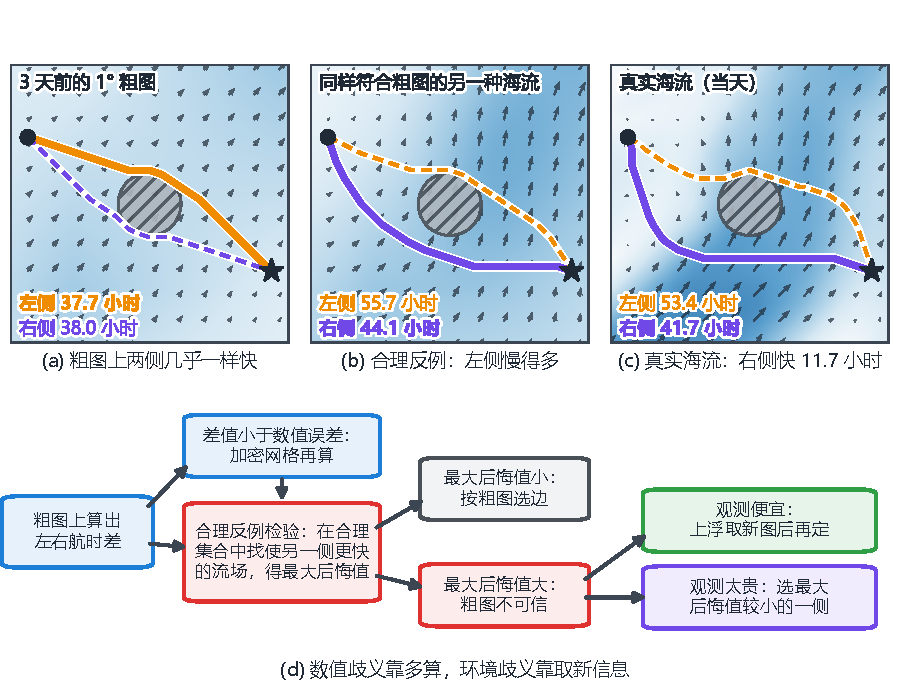
\includegraphics[width=\linewidth]{fig_route_overview}
\caption{粗图下的选边决策与合理反例检验（2022年1月18日测试任务）。(a) 3天前的1°粗图：左侧37.7小时、右侧38.0小时，按粗图选左侧；(b) 合理集合中搜出的合理反例：左侧55.7小时、右侧44.1小时；(c) 当天真实海流：右侧快11.7小时；(d) 本文的决策流程。加算只能把(a)中0.3小时的差值算得更准，合理反例检验则把(b)这样与粗图同样相容、却要求选另一侧的海流显式找出来。}
\label{fig:overview}
\end{figure}

最直接的做法是多算，但当缺失的是环境信息时，多算只会让答案更精细，而不会更正确。加密求解网格、增加航向离散度或增加规划器的推演次数\cite{lolla2014levelset}，只能减小同一张粗图上的离散误差，不能补充粗图缺失的涡旋与切变；规划器在有偏的内部模型上搜索得越久，越会把模型误差当作机会，对自身方案的估值越高\cite{smith2006curse,jiang2015horizon,cuadron2025overthinking}。作者在前期的东海赤潮巡测研究中观察到了这一现象（图\ref{fig:curse}）：航行器携带3天前的卫星叶绿素图，每次决策的推演从64次增至20万次，规划器对自身航线的估值从0.762持续升至0.917，而航线的真实价值约2000次推演后便不再提高。

\begin{figure}[t]
\centering
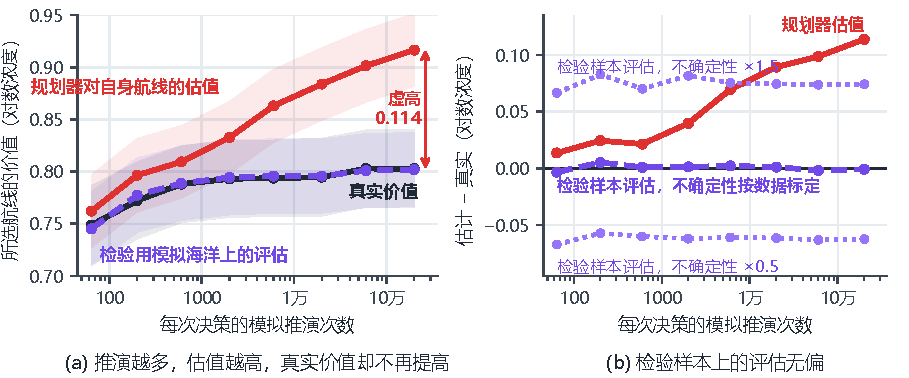
\includegraphics[width=\linewidth]{fig_curse}
\caption{前期东海赤潮巡测研究中的过度计算现象。(a) 所选航线的价值随每次决策推演次数的变化：规划器对自身航线的估值持续上升，真实价值与检验用模拟海洋上的评估约2000次后不再提高；(b) 估值减真实价值：规划器自身估值的高估随计算量增大，检验用模拟海洋上的评估保持无偏。多算让答案更精细，却不提供区分不同真实海洋的新信息。}
\label{fig:curse}
\end{figure}

第二种做法是把海流的不确定性纳入规划，但随机样本既难以估准关键方向上的效应，也不回答何时该去观测。集合规划在若干随机扰动流场（集合成员）上评估两侧航时，按集合平均选边或统计改变选边的成员比例\cite{wang2016path,subramani2018stochastic,kularatne2018forecast}。有限样本的平均受抽样误差左右；改变选边的成员比例只记录有多少成员改选，不度量改选后会多花多少时间，因而难以区分多花半小时与多花十几小时的任务\cite{benhaim2006infogap,marx2020predictive}。更重要的是，这类方法把不确定性当作固定输入，并不判断何时应停止计算、转而观测\cite{horvitz1987reasoning,russell1991right,lin2015metareasoning,elboher2023formal}。

第三种做法是主动观测，但为全场重构而采集的数据未必有助于选边。自适应采样引导航行器前往不确定性最高的海区，以降低全场估计误差\cite{srinivas2012gpucb,hollinger2014sampling,fossum2019}；然而，若某处误差对左右两侧的影响相同，测量它只是徒耗航时，若决定两侧快慢的切变远在数十千米之外，起点附近的测量也改变不了判断。序贯实验设计与模型判别理论指出，观测的价值在于区分要求不同行动的竞争假设\cite{chernoff1959sequential,box1967discrimination,garivier2016optimal,attia2018goal}。对选边而言，真正需要回答的问题因此是：与粗图同样相容的海流中，是否存在一个使另一侧更快的流场？它会让当前选择多花多少时间？

本文据此提出合理反例检验，其核心思想是：两侧难分高下有两种性质不同的原因，应分别交给计算与观测（图\ref{fig:overview}(d)）。若只是求解网格过粗、两侧航时差小于求解误差（数值歧义），加密计算即可看清粗图的本意；若粗图同时容许“左侧更快”与“右侧更快”的真实海流（环境歧义），算得再细也无法分辨，只能补充新信息。为区分二者，我们用多年再分析数据统计粗图的误差，划定与粗图相容的合理流场集合（合理集合），在其中搜索使另一侧更快的流场（合理反例），并计算坚持当前选择最多会多花的航时（最大后悔值）；最大后悔值超过阈值时，判定粗图对本次决定不可信，转而获取新信息。由于航时对流场的导数可以沿当前最快航线直接累加，这一检验只需数十次航线求解，适合在端侧运行。

本文的主要贡献有三点：
\begin{itemize}
    \item \textbf{区分数值歧义与环境歧义的决策判据。}据我们所知，本文首次在航行器航路决策中把“继续计算还是去观测”转化为一个可计算的问题——与粗图相容的海流中能否找到使另一侧更快的合理反例——并以最大后悔值衡量其代价：数值歧义交给计算，环境歧义交给观测。
    \item \textbf{由海洋大数据标定的合理集合与高效反例搜索。}合理集合的误差大小、空间相关长度与半径均由多年再分析误差标定；基于包络定理的梯度使每次迭代只需两次最短路求解，约71次求解即达到随机抽样2048次求解的选边效果。
    \item \textbf{跨海区与真实卫星图的系统验证。}在黑潮、湾流、阿古拉斯回流区以及改带卫星测高地转流图四种设置的逾两千个测试任务上，加算几乎不改变选错率，按最大后悔值排名前20\%的任务集中了53\%--71\%的额外航时；在粗图误差大的海区，被判定不可信后上浮取图使平均额外航时降低六成以上。
\end{itemize}

第\ref{sec:related}节回顾相关工作；第\ref{sec:problem}节建立问题模型并分析选边决策的难点；第\ref{sec:method}节给出合理反例检验方法；第\ref{sec:exp}节报告实验结果；第\ref{sec:innovation}节拆解本文的原创创新点与研究脉络；第\ref{sec:conclusion}节总结全文。

\section{相关工作}
\label{sec:related}

合理反例检验涉及三方面的研究：不确定海流中的航路规划、元推理与计算的价值，以及面向决策的信息获取。

\subsection{不确定海流中的航路规划}
确定性海流中的时间最优航线可由图搜索或水平集方法求得\cite{dijkstra1959note,lolla2014levelset}，区域海洋模式的预报也已用于引导航行器追踪演变中的海洋过程\cite{smith2010planning}。为应对预报的不确定性，研究者发展了集合规划\cite{wang2016path}、基于随机动态正交水平集方程的时间最优规划\cite{subramani2018stochastic}，以及计入预报不确定性的图搜索规划\cite{kularatne2018forecast}；数据同化则用集合卡尔曼滤波等方法把新观测并入海流估计\cite{anderson2001eakf}。这些方法或假设海流图准确，或在给定的集合成员上求期望最优，都没有判断一张海流图何时对某个具体决定不可信。

\subsection{元推理与计算的价值}
元推理研究计算本身的价值，以决定何时停止思考、开始行动\cite{horvitz1987reasoning,russell1991right}；在机器人规划中，这一思想体现为学习停止规则、自适应分配计算预算，以及让规划与执行并行\cite{xiao2020thinking,sung2021quit,lin2015metareasoning,elboher2023formal,magnino2026metareasoning}。然而，在有误差的模型上择优，选中方案的价值往往被高估，即决策分析中的优化者诅咒\cite{smith2006curse}；模型越不准，有效的规划步长越短\cite{jiang2015horizon}。智能体推理的研究也发现，外部状态未知时，增加推理计算不能代替与环境交互\cite{hunt2021formalizing,shen2025thinking,kobalczyk2025active,cuadron2025overthinking}。这些工作决定何时停止计算，却默认继续计算总能改善决策；本文检验的正是这一前提何时不成立。

\subsection{面向决策的信息获取}
只有能区分竞争假设、并可能改变行动的观测才有决策价值\cite{chernoff1959sequential,box1967discrimination}。最优臂识别、信息导向采样与目标导向实验设计都针对具体决策采集样本，而不是均匀降低全局方差\cite{garivier2016optimal,russo2018thompson,russo2018ids,attia2018goal}；面向全场估计的自适应采样则引导航行器前往不确定性高的海区\cite{srinivas2012gpucb,hollinger2014sampling,fossum2019}。鲁棒决策与预测多解性研究进一步主张，当多个与数据相容的模型给出相反结论时，应考察不确定集内的最坏表现\cite{benhaim2006infogap,marx2020predictive}。本文把这一思想用于连续海流场：不确定集由多年误差数据标定，并用梯度直接搜索使选边翻转的流场。

\subsection{本文与已有工作的区别}
\label{sec:diff}
综上，已有工作分别解决了求最快航线、刻画海流的不确定性和获取新信息的问题，但没有回答一张海流图何时对某个具体决定不可信、何时值得付出观测的代价。表\ref{tab:innovation}逐项列出本文三个创新点与已有做法的区别、支持它们的实验证据，以及各自的适用条件。

\begin{table}[!htb]
\centering
\caption{原创创新点拆解：已有做法、本文做法、实验证据与适用条件。}
\label{tab:innovation}
\footnotesize
\setlength{\tabcolsep}{4pt}
\begin{tabular}{@{}>{\raggedright\arraybackslash}p{0.13\linewidth}>{\raggedright\arraybackslash}p{0.20\linewidth}>{\raggedright\arraybackslash}p{0.21\linewidth}>{\raggedright\arraybackslash}p{0.24\linewidth}>{\raggedright\arraybackslash}p{0.14\linewidth}@{}}
\toprule
创新点 & 已有做法及其不足 & 本文做法 & 实验证据 & 适用条件 \\
\midrule
1. 以合理反例判定该计算还是该观测 & 加密网格与元推理只减小求解误差，默认海流图准确；集合规划不回答何时转而观测。 & 以合理集合中的最大后悔值判定风险的来源：求解误差交给计算，粗图误差交给观测。 & 图\ref{fig:compute}：四种设置中计算量增加64倍，选错率的变化不超过2个百分点，换用当天0.5°图后降至7.0\%--10.4\%；81.0\%--99.7\%的决定存在合理反例。 & 单个禁航区的左右选边；单次任务中海流视为定常。 \\
\addlinespace
2. 数据标定的合理集合与包络定理梯度搜索 & 鲁棒方法的不确定集由分析者给定；集合方法需上千个成员才能估准，改选比例不计代价。 & 用多年误差标定误差大小、相关长度与半径；沿最快航线累加导数，每次迭代求解2次。 & 图\ref{fig:rank}、\ref{fig:budget}：约71次求解达到2048次求解的选边效果；前20\%的任务占53\%--71\%的额外航时；改用相似日差值构造集合后，保守改选不再有效（表\ref{tab:scope}）。 & 依赖开发年份的误差统计；流场变化大时一阶近似有误差。 \\
\addlinespace
3. 以最大后悔值决定何时观测 & 自适应采样为降低全场误差而测量；或一律观测，或从不观测。 & 最大后悔值超过阈值才观测，优先上浮取图；不能观测时改选最大后悔值较小的一侧。 & 图\ref{fig:respond}：湾流与阿古拉斯回流区的平均额外航时降至1.31与2.20小时；黑潮中保守改选从0.98降至0.70小时。 & 保守改选要求两侧最坏情形差别分明；黑潮中上浮代价需低于约0.8小时。 \\
\bottomrule
\end{tabular}
\end{table}

\section{问题建模与分析}
\label{sec:problem}

本节先给出任务、航线求解与合理流场集合的模型，再分析粗图下选边的难点，并由此导出方法的三条原则。

\subsection{任务场景与数据}
本文研究航行器携带粗图绕越禁航区时的左右选边。主设置取台湾以东至东海的黑潮区（23°--31°N、121°--129°E），采用HYCOM全球再分析10米深度的1/12°流速场\cite{chassignet2007hycom}，2019年1月1日至2024年8月29日每3天一张快照，共689张；2019--2021年为开发年份，用于标定全部参数，2022--2024年为测试年份，只评价一次。每张快照生成2个任务：起终点相距100--140千米，两点中间设半径15千米的禁航区，只保留粗图上平均流速不低于0.3米/秒的强流任务。航行器携带3天前的1°粗图（格内平均），当天的1/12°场作为真实海流（表\ref{tab:settings}）。为检验结论的适用范围，我们在湾流与阿古拉斯回流区重复了同一流程，并在黑潮区让航行器改带美国国家海洋和大气管理局的近实时融合卫星测高地转流图。

\begin{table}[tb]
\centering
\caption{黑潮主设置的实验设置与参数（其余设置只换海区或粗图来源，参数各自在开发年份标定）。}
\label{tab:settings}
\small
\begin{tabular}{@{}p{0.16\linewidth}p{0.80\linewidth}@{}}
\toprule
项目 & 设置 \\
\midrule
海流数据 & HYCOM 全球海洋再分析（GLBy0.08，实验 93.0），水平分辨率 1/12°，取 10 米深度；23°--31°N、121°--129°E（台湾以东至东海，含黑潮）；2019-01-01 至 2024-08-29 每 3 天 12:00 时一张，共 689 张 \\
任务 & 每张快照抽 2 个：起终点相距 100--140 千米、离岸不少于 20 千米，两点中间设半径 15 千米的禁航区，可从左侧或右侧绕过；只取粗图上任务区平均流速不低于 0.3 米/秒的强流任务；开发 710 个（2019--2021 年），测试 623 个（2022--2024 年） \\
粗图与真实海流 & 航行器带 3 天前的 1° 粗分辨率海流图（下称粗图，格内平均）；真实海流为当天 1/12° 再分析海流场 \\
航行器 & 对水速度 1.0 米/秒；选定一侧后，按真实海流在该侧以最快方式航行 \\
航线求解 & 网格最短路：粗网格求解 8 千米网格、8 个方向；中网格求解 4 千米、16 个方向；细网格求解 2 千米、32 个方向（计算量之比 1 : 8 : 64）；顶流过强的边不可通行 \\
合理流场集合 & 粗图加上由流函数生成的无散误差模态的组合，各点误差大小与相关长度（76 千米）由开发年份标定，组合系数服从标准正态；半径 $r=1.5$（开发年份中包住真实左右航时差的任务占 93\%） \\
合理反例检验 & 在半径 $r$ 的球内对左右航时差做投影梯度上升（梯度沿最快航线累加）；两个方向、半径 1 与 2 各搜一次，其他半径线性插值，每个任务约 71 次中网格求解 \\
观测方式 & 原地停留测流（出发前 2 小时测 12 次）；沿途测流 30 千米或沿途测流 60 千米后可换边；绕行定点测流（去前方 40 千米内反例与粗图差别最大处测量）；上浮取当天 1° 图或上浮取当天 0.5° 图（每次 1 小时）；测流噪声 0.05 米/秒 \\
阈值判据 & 最大后悔值超过 8 小时（开发年份选定）时判定粗图不可信，触发超阈值时保守改选或超阈值时上浮取图，否则按粗图选边 \\
评价指标 & 额外航时 = 实际航时 $-$ 真实更快一侧的航时（小时）；配对差值的 95\% 置信区间按天整组自助重抽样 2000 次 \\
\bottomrule
\end{tabular}

\end{table}

\subsection{航线求解}
给定水平海流场 $\boldsymbol{u}(\boldsymbol{x})$ 与航行器恒定的对水速度 $V = 1.0$ 米/秒，选定绕行一侧 $s \in \{\text{L}, \text{R}\}$（左侧或右侧）后的最快航线由有向图最短路算法求取\cite{dijkstra1959note}。对长度为 $\ell_e$、单位方向为 $\boldsymbol{d}_e$ 的有向边 $e$，记沿边流速分量为 $u_{\parallel} = \boldsymbol{u} \cdot \boldsymbol{d}_e$、垂直边分量为 $u_{\perp} = \|\boldsymbol{u} - u_{\parallel}\boldsymbol{d}_e\|$（边上的流速取两端节点的平均），则航行器的对地速度 $v_{\text{g}}(e)$ 与通行时间 $t(e)$ 为
\begin{equation}
v_{\text{g}}(e) = u_{\parallel} + \sqrt{V^2 - u_{\perp}^2}, \qquad t(e) = \frac{\ell_e}{v_{\text{g}}(e)}.
\label{eq:edge_time}
\end{equation}
当 $|u_{\perp}| \ge V$ 或 $v_{\text{g}}(e) \le 0$ 时该边不可通行。在禁航区左侧或右侧的子图上分别求最短路，得两侧最快航时 $T_{\text{L}}(\boldsymbol{u})$、$T_{\text{R}}(\boldsymbol{u})$ 及左右航时差
\begin{equation}
\Delta T(\boldsymbol{u}) = T_{\text{L}}(\boldsymbol{u}) - T_{\text{R}}(\boldsymbol{u}),
\label{eq:delta_t}
\end{equation}
$\Delta T(\boldsymbol{u}) < 0$ 表示左侧更快。求解分粗网格（8千米、8个方向）、中网格（4千米、16个方向）与细网格（2千米、32个方向）三档，计算量之比为 $1:8:64$。选定一侧后，假设航行器按真实海流 $\boldsymbol{u}_{\text{true}}$ 在该侧以最快方式航行，以便专门评价选边这一顶层决策。

\subsection{合理流场集合}
粗图 $\boldsymbol{u}_0(\boldsymbol{x})$ 的误差成片出现（图\ref{fig:data}），因此我们用空间相关的无散模态而非逐点独立的扰动描述它。以流函数生成误差模态，按历史误差逐点缩放（缩放后近似无散），构造与粗图相容的流场
\begin{equation}
\boldsymbol{u}(\boldsymbol{x}; \boldsymbol{z}) = \boldsymbol{u}_0(\boldsymbol{x}) + \sum_{k=1}^{K} z_k \boldsymbol{m}_k(\boldsymbol{x}), \qquad \boldsymbol{m}_k(\boldsymbol{x}) = \mathbf{S}(\boldsymbol{x})\, \nabla^{\perp}\phi_k(\boldsymbol{x}),
\label{eq:plausible_field}
\end{equation}
其中 $\nabla^{\perp} = (-\partial_y, \partial_x)$，$\{\phi_k\}_{k=1}^{K}$ 为相关长度 $L_{\text{corr}}$ 的高斯相关流函数的前 $K$ 个主模态（保留95\%方差），$\mathbf{S}(\boldsymbol{x})$ 为逐点误差标准差构成的对角矩阵，系数 $\boldsymbol{z} = (z_1, \dots, z_K)^{\top}$ 先验服从标准正态分布。给定半径 $r > 0$，合理流场集合（合理集合）定义为以粗图为中心的不确定集
\begin{equation}
\mathcal{U}(r) = \left\{ \boldsymbol{u}(\boldsymbol{x}; \boldsymbol{z}) \;\middle|\; \|\boldsymbol{z}\|_2 \le r \right\}.
\label{eq:plausible_set}
\end{equation}

\begin{figure}[tb]
\centering
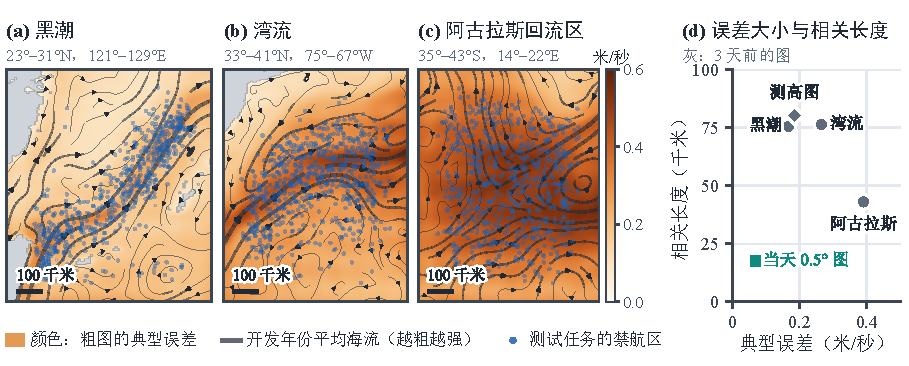
\includegraphics[width=\textwidth]{route3_data}
\caption{三个研究海区与3天前粗图的误差（开发年份）。(a)--(c) 黑潮、湾流与阿古拉斯回流区：底色为3天前1°粗图相对真实海流的典型误差，黑线为平均海流，蓝点为测试任务的禁航区；(d) 各设置所用海流图的典型误差与误差的空间相关长度。3天前的图误差大且成片相关，相关长度与航线尺度相当；当天的0.5°图误差小、相关范围短。}
\label{fig:data}
\end{figure}

\subsection{可选行动与评价指标}
航行器面对粗图有三类行动。一是在同一张粗图上加算，即从粗网格求解改为中网格或细网格求解；在粗图上用细网格求解并选更快一侧，作为基线（按粗图选边）。二是不取新信息、改用其他选边准则，如集合平均选边（在随机抽取的集合成员上选平均航时更短的一侧）或选最大后悔值较小的一侧。三是获取新信息，包括原地停留测流（2小时测12次）、沿途测流30或60千米后再决定是否换边、绕行到指定点测流，以及上浮获取当天的1°或0.5°海流图（每次计1小时）；测得的流速按线性高斯更新修正模态系数。评价指标为额外航时，即实际总航时 $T_{\text{total}}$ 减去真实更快一侧的航时：
\begin{equation}
\mathcal{L} = T_{\text{total}} - \min\left\{ T_{\text{L}}(\boldsymbol{u}_{\text{true}}),\, T_{\text{R}}(\boldsymbol{u}_{\text{true}}) \right\}.
\label{eq:loss}
\end{equation}

\subsection{问题分析}
\label{sec:analysis}
粗图下的选边之所以困难，在于两侧航时接近有两种不同的原因，而观测又各有代价与视野。第一，求解误差与粗图误差混在一起：同一张粗图上，粗网格与细网格求得的左右航时差可相差3.2小时（开发年份的95\%分位数），仅看航时差无法判断该加算还是该观测。第二，粗图误差在空间上大范围相关，各设置的相关长度为43--80千米，与航线尺度相当（图\ref{fig:data}(d)）；一个误差模态就能使整条左侧或右侧通道同时顺流或逆流，因此与粗图同样相容、却要求选另一侧的海流应当普遍存在，“有没有反例”本身难以区分任务的风险高低，需要度量反例会让当前选择多花多少时间。第三，观测的视野与代价不同：就地测流只能看到航线附近，而决定两侧快慢的切变可能远在数十千米之外；上浮取图能同时更新两侧的海流，却要中断航行约1小时。

这三点决定了方法的三条原则（第\ref{sec:method}节）：只在航时差小于求解误差时加算，以排除数值歧义；以最大后悔值而非反例的有无衡量环境歧义；只在最大后悔值超过阈值时付出观测的代价，并优先选用能同时更新两侧的观测。

\section{合理反例检验}
\label{sec:method}

合理反例检验按第\ref{sec:analysis}节的三条原则组织（算法\ref{alg:counterexample_gate}）：按需细网格求解，排除数值歧义（第\ref{sec:numeric}节）；在由数据标定的合理集合（第\ref{sec:calib}节）中用梯度搜索最大后悔值，衡量环境歧义（第\ref{sec:search}节）；按阈值判据决定是否付出观测的代价（第\ref{sec:gate}节）。

\begin{algorithm}[t]
\caption{基于合理反例检验的选边决策}
\label{alg:counterexample_gate}
\begin{algorithmic}[1]
\Require 粗图 $\boldsymbol{u}_0$，误差模态 $\{\boldsymbol{m}_k\}_{k=1}^{K}$，半径 $r$，数值误差容限 $\tau_{\text{num}}$，阈值 $\theta$，单次上浮代价 $c_{\text{surf}}$ 与平衡点 $c^*$。
\Ensure 绕行一侧 $s^*$。
\State 在 $\boldsymbol{u}_0$ 上作粗网格求解，得左右航时差 $\Delta T_{\text{coarse}}(\boldsymbol{u}_0)$。
\If{$|\Delta T_{\text{coarse}}(\boldsymbol{u}_0)| < \tau_{\text{num}}$}
    \State 改用细网格求解，$s_0 \gets \arg\min_{s} T_s^{\text{fine}}(\boldsymbol{u}_0)$。\Comment{排除数值歧义}
\Else
    \State $s_0 \gets \arg\min_{s} T_s^{\text{coarse}}(\boldsymbol{u}_0)$。
\EndIf
\State 在 $\boldsymbol{z}=\boldsymbol{0}$ 处求左右最快航线，按式(\ref{eq:envelope_grad})得梯度 $\boldsymbol{g}(\boldsymbol{0})$。
\State 沿 $\pm\boldsymbol{g}(\boldsymbol{0})$ 跳至球面并作投影梯度上升，得 $R_{\text{L}}(r)$ 与 $R_{\text{R}}(r)$。\Comment{衡量环境歧义}
\If{$R_{s_0}(r) \le \theta$}
    \State \Return $s^* \gets s_0$。\Comment{粗图可信}
\ElsIf{允许上浮且 $c_{\text{surf}} < c^*$}
    \State 上浮获取当天0.5°图 $\boldsymbol{u}_{\text{new}}$，\Return $s^* \gets \arg\min_{s} T_s(\boldsymbol{u}_{\text{new}})$。\Comment{取新信息}
\Else
    \State \Return $s^* \gets \arg\min_{s} R_s(r)$。\Comment{保守改选}
\EndIf
\end{algorithmic}
\end{algorithm}

\subsection{按需细网格求解：只在航时差小于求解误差时加算}
\label{sec:numeric}
一律使用细网格求解能消除离散误差，但计算量是粗网格的64倍，对两侧本就相差十几小时的任务并无必要；一律使用粗网格，又会在两侧接近时被折线误差误导。因此，我们只在可能存在数值歧义时加算。在开发年份比较同一张粗图上粗网格与细网格求得的左右航时差，取二者差值绝对值的95\%分位数作为数值误差容限 $\tau_{\text{num}}$（黑潮主设置为3.2小时）；在线决策时先作粗网格求解，仅当 $|\Delta T_{\text{coarse}}(\boldsymbol{u}_0)| < \tau_{\text{num}}$ 时改用细网格求解，由此确定粗图的选边 $s_0$。

\subsection{合理集合的数据标定：让“合理”由多年误差决定}
\label{sec:calib}
合理集合界定了“与粗图同样相容”的范围，它的形状与大小直接决定检验的结论。凭经验设定不确定集，或直接借用历史上相似日期的小尺度差，都会偏离粗图误差的真实结构，后者在第\ref{sec:scope}节的消融实验中使检验失去作用。因此，我们用开发年份中“粗图减真实海流”的误差标定合理集合，分两步进行。第一步，统计各网格点误差的标准差，得到式(\ref{eq:plausible_field})中的 $\mathbf{S}(\boldsymbol{x})$（黑潮主设置全区中位数为0.17米/秒），并由误差的空间相关衰减定出相关长度 $L_{\text{corr}}$（黑潮主设置为76千米）。第二步，在开发年份的任务上寻找最小的半径，使合理集合给出的左右航时差范围包住真实左右航时差的任务不少于90\%，得 $r = 1.5$（开发年份覆盖93\%，测试年份覆盖94\%）。

\subsection{最大后悔值的梯度搜索}
\label{sec:search}
判断粗图的选择 $s_0$ 是否面临环境歧义，需要求出合理集合中坚持 $s_0$ 最多会多花的航时。在流场 $\boldsymbol{u}(\boldsymbol{z}) \in \mathcal{U}(r)$ 下，选一侧 $s$ 比另一侧 $\bar{s}$ 多花的航时称为后悔值，其在合理集合内的最大值即最大后悔值：
\begin{equation}
R_s(r) = \max_{\|\boldsymbol{z}\|_2 \le r} J_s(\boldsymbol{z}), \qquad J_s(\boldsymbol{z}) = \max\left\{ 0,\, T_s(\boldsymbol{u}(\boldsymbol{z})) - T_{\bar{s}}(\boldsymbol{u}(\boldsymbol{z})) \right\}.
\label{eq:worst_regret}
\end{equation}
$R_{s_0}(r) > 0$ 意味着存在使另一侧更快的合理反例，其大小给出坚持 $s_0$ 的最大代价；图\ref{fig:example}(b)即示例任务在标定半径处搜出的合理反例。

求最大后悔值的常规做法有两种：随机抽取集合成员，或用有限差分求航时差对模态系数的导数。前者要大量样本才能把少数关键方向上的效应估准（第\ref{sec:budget}节），后者每次迭代需要 $2K$ 次最短路求解。我们利用最优化中的包络定理避开这两种代价：流场作微小变化时，最快航线 $P_s^*(\boldsymbol{z})$ 的节点序列在一阶近似下不变，因此航时对系数 $z_k$ 的导数等于沿当前最快航线累加各边通行时间对流速的导数，
\begin{equation}
\frac{\partial T_s}{\partial z_k} = \sum_{e \in P_s^*(\boldsymbol{z})} \left( \frac{\partial t(e)}{\partial u_{\parallel}} \boldsymbol{d}_e + \frac{\partial t(e)}{\partial u_{\perp}} \boldsymbol{n}_e \right) \cdot \frac{\boldsymbol{m}_k(\boldsymbol{x}_e^{-}) + \boldsymbol{m}_k(\boldsymbol{x}_e^{+})}{2},
\label{eq:envelope_grad}
\end{equation}
其中 $\boldsymbol{x}_e^{-}$、$\boldsymbol{x}_e^{+}$ 为边 $e$ 的两端节点，$\boldsymbol{n}_e$ 为垂直边方向的单位向量，标量导数由式(\ref{eq:edge_time})直接给出：
\begin{equation}
\frac{\partial t(e)}{\partial u_{\parallel}} = -\frac{\ell_e}{v_{\text{g}}(e)^2}, \qquad \frac{\partial t(e)}{\partial u_{\perp}} = \frac{\ell_e u_{\perp}}{v_{\text{g}}(e)^2 \sqrt{V^2 - u_{\perp}^2}}.
\label{eq:edge_deriv}
\end{equation}
于是每次迭代只需在中网格上求左右两条最快航线（2次求解），即可得到对全部 $K$ 个系数的梯度 $\boldsymbol{g}(\boldsymbol{z}) = \nabla_{\boldsymbol{z}} \Delta T(\boldsymbol{u}(\boldsymbol{z}))$。搜索从粗图 $\boldsymbol{z}=\boldsymbol{0}$ 出发，先沿 $\pm\boldsymbol{g}(\boldsymbol{0})$ 一步跳到球面 $\|\boldsymbol{z}\|_2 = r$（若航时差随流场线性变化，这一步已是精确解），再以步长减半的投影梯度上升细化。我们在半径1与2上各搜索一次，其他半径按线性插值，每个任务平均约71次中网格求解。

\subsection{阈值判据：粗图不可信时先取新信息}
\label{sec:gate}
总是观测会在大多数本无风险的任务上浪费时间，从不观测又会在少数高风险任务上多花数小时。因此，我们只在最大后悔值超过阈值 $\theta$ 时判定粗图不可信，并付出观测的代价；$\theta$ 在开发年份按平均额外航时最小选定，黑潮主设置为8小时。具体而言，若 $R_{s_0}(r) \le \theta$，按粗图选边 $s_0$；若 $R_{s_0}(r) > \theta$，在单次上浮代价低于平衡点 $c^*$ 时上浮获取当天0.5°海流图并按新图选边（超阈值时上浮取图），能同时更新两侧的海流；不能上浮或代价过高时，改选最大后悔值较小的一侧（超阈值时保守改选）：
\begin{equation}
s_{\text{cons}} = \arg\min_{s \in \{\text{L}, \text{R}\}} R_s(r).
\label{eq:conservative_choice}
\end{equation}
保守改选等价于按合理集合给出的左右航时差范围的中点选边：若航时差随流场线性变化，这一中点就是粗图的航时差，二者选择相同；只有当一侧的最不利情形比另一侧严重得多时，才会改选。

\section{实验}
\label{sec:exp}

本节依次检验第\ref{sec:method}节的三个选择：加算能否消除选边错误（第\ref{sec:compute}节）；最大后悔值能否找出高风险任务、梯度搜索是否高效（第\ref{sec:rank}、\ref{sec:budget}节）；判定粗图不可信后应如何行动（第\ref{sec:respond}节）。第\ref{sec:scope}节考察换海区与换地图时结论的适用范围。

\subsection{实验设置}
全部参数在开发年份（2019--2021年）标定，在测试年份（2022--2024年）只评价一次。主设置为黑潮区（测试任务623个）；为检验结论的适用范围，我们在湾流（33°--41°N、75°--67°W，643个）与阿古拉斯回流区（35°--43°S、14°--22°E，618个）重复了同一流程，并在黑潮区让航行器改带美国国家海洋和大气管理局的近实时融合卫星测高地转流图（0.25°，3天前，648个）；后两种设置的检验内容在获取数据之前即已确定。对比方法包括：同一张粗图上的粗、中、细网格求解（细网格求解即基线）；集合平均选边（32个集合成员）与选最大后悔值较小的一侧；四种就地测流；总是上浮取当天1°或0.5°图；以及本文的超阈值时上浮取图与超阈值时保守改选。与基线的配对差按天整组重抽样（2000次）求95\%置信区间，区间不含0时称差异显著。

\subsection{加算消除不了环境歧义}
\label{sec:compute}
在同一张粗图上增加计算，只能纠正很少一部分选边错误。在黑潮测试年份，从粗网格求解改为细网格求解，计算量增加64倍，改变了64个任务的选择，其中38个改对、26个改错，选错率仅从21.7\%降至19.7\%；换成当天0.5°图，选错率则降至10.4\%（图\ref{fig:ambiguity}(a)）。其余三种设置中，加算前后选错率的变化都不超过1个百分点。

\begin{figure}[t]
\centering
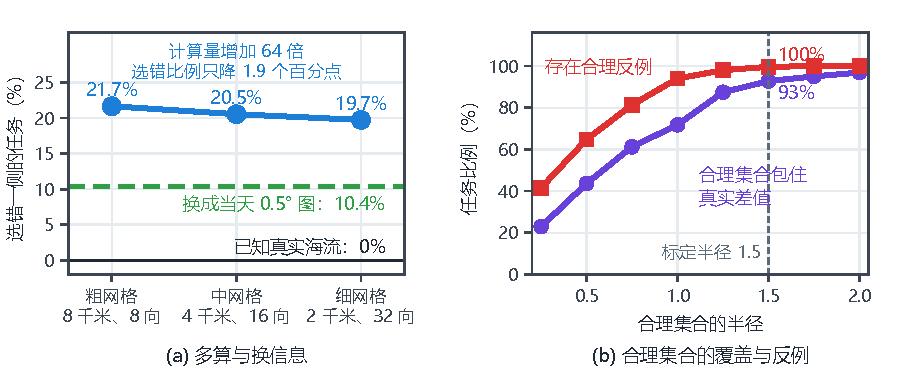
\includegraphics[width=0.92\linewidth]{fig_route_ambiguity}
\caption{求解计算量与环境信息对选边错误的不同作用（黑潮测试年份）。(a) 选错一侧的任务比例：粗网格、中网格、细网格求解依次为21.7\%、20.5\%、19.7\%，换成当天0.5°图降至10.4\%；(b) 随合理集合半径增大，合理集合包住真实左右航时差的任务比例（开发年份）与存在合理反例的任务比例（测试年份）。加算只能消除很少一部分错误；在足以包住真实海流的合理集合中，几乎每个决定都存在合理反例。}
\label{fig:ambiguity}
\end{figure}

加算无效的原因在于环境歧义普遍存在。在覆盖94\%真实左右航时差的标定半径下，黑潮99.7\%的测试任务都能找到合理反例（图\ref{fig:ambiguity}(b)），湾流与阿古拉斯回流区也分别为98.8\%与99.2\%。这些任务的粗图本身容许两种相反的选择，求解得再细也无法从中分辨；因此，“有没有合理反例”不足以区分任务，需要看反例会让当前选择多花多少时间。

\subsection{最大后悔值找得出额外航时所在}
\label{sec:rank}
按最大后悔值排序，能把大部分额外航时集中到少数任务上。黑潮测试年份的额外航时高度集中，额外航时最大的10\%任务占全部额外航时的92\%；按最大后悔值排在前20\%的任务占67\%，而按改变选边的成员比例排序只占49\%，按粗图左右航时差排序只占34\%（图\ref{fig:risk}(a)）。在湾流、阿古拉斯回流区与改带卫星测高地转流图时，最大后悔值排在前20\%的任务分别占71\%、53\%与67\%，均高于改变选边的成员比例（49\%、36\%与52\%）。

\begin{figure}[t]
\centering
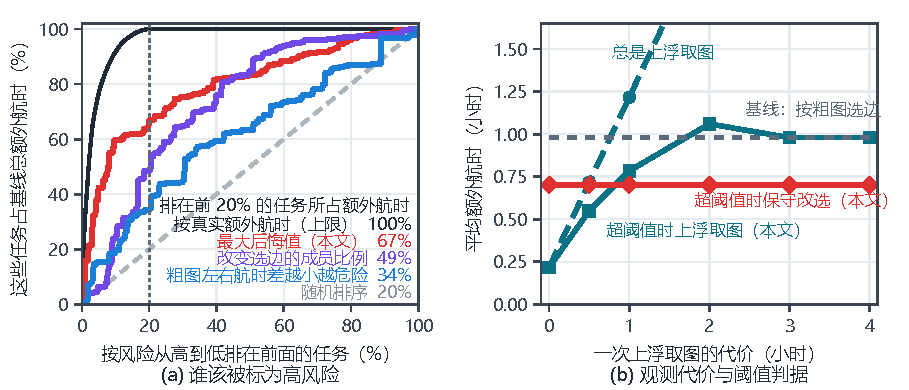
\includegraphics[width=0.92\linewidth]{fig_route_risk}
\caption{最大后悔值的风险排序与上浮代价（黑潮测试年份）。(a) 按不同指标从高到低排序时，排在前面的任务累计所占的额外航时；(b) 平均额外航时随单次上浮取当天0.5°图的代价的变化。最大后悔值把大部分额外航时集中到少数任务上；单次上浮代价低于约1小时时，超阈值时上浮取图最优。}
\label{fig:risk}
\end{figure}

这一优势来自度量的对象，而不是样本的多少。改变选边的成员比例只数有多少集合成员改选，把多花半小时与多花十几小时等同看待；最大后悔值则直接度量改选的代价。即使集合成员增至1024个，按改变选边的成员比例排在前20\%的任务也只占44\%，而在同一批成员上计算的后悔值的集合平均可达67\%（图\ref{fig:budget}(b)）。在黑潮主设置中，阈值判据（$\theta=8$小时）标记了47\%的任务，这些任务囊括了82\%的额外航时。

\subsection{梯度搜索以约二十九分之一的求解次数达到同样的选边效果}
\label{sec:budget}
在决定选哪一侧时，梯度搜索约71次航线求解，即达到集合平均选边使用1024个集合成员（2048次求解）的效果（图\ref{fig:budget}(a)）。选最大后悔值较小的一侧，等价于按合理集合给出的左右航时差范围的中点选边：若航时差随流场线性变化，这一中点就是粗图的航时差，二者选择相同；只有一侧的最不利情形比另一侧严重得多时，才会改选。

\begin{figure}[t]
\centering
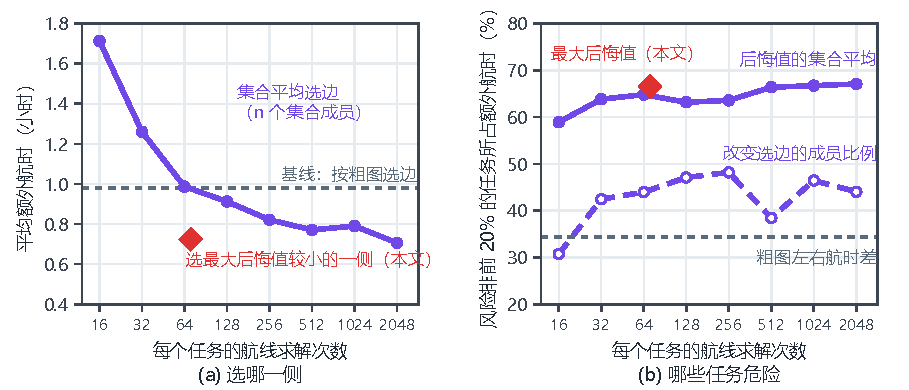
\includegraphics[width=0.92\linewidth]{fig_route_budget}
\caption{集合成员数量与梯度搜索的比较（黑潮测试年份）。(a) 平均额外航时随每个任务航线求解次数的变化：曲线为集合平均选边，菱形为梯度搜索后选最大后悔值较小的一侧；(b) 排在前20\%的任务所占的额外航时：曲线为在相同集合成员上计算的后悔值的集合平均与改变选边的成员比例，菱形为最大后悔值。选对一侧要上千个集合成员才能估准，梯度搜索约71次求解即可做到；排序的优劣则取决于是否度量多花的时间。}
\label{fig:budget}
\end{figure}

集合平均选边估计的是同一个修正量，却受抽样误差左右。32个集合成员时，集合平均的抽样误差（中位数2.4小时）大于它要估计的修正量（中位数1.7小时），改选多由噪声驱动，平均额外航时为0.99小时，显著高于梯度搜索后保守选边的0.72小时；集合成员增至数百个以上，二者才不再有显著差异。对算力有限的航行器而言，梯度搜索省下的正是这上千次航线求解。

\subsection{判定粗图不可信后，取新信息最划算}
\label{sec:respond}
对被阈值判据标记的任务，最划算的回应是获取新信息，在粗图误差大的海区尤其如此。湾流与阿古拉斯回流区的粗图误差大，基线的平均额外航时分别为3.56小时与6.87小时；即使每次上浮计1小时，超阈值时上浮取图仍使二者显著降至1.31小时与2.20小时（表\ref{tab:scope}）。在湾流，它只在约三分之二的任务上上浮，就优于总是上浮（1.53小时）；在阿古拉斯回流区，粗图误差普遍较大，总是上浮（1.98小时）略好于按阈值上浮。在黑潮主设置中，单次上浮代价低于约1小时时，超阈值时上浮取图是最优回应（图\ref{fig:risk}(b)）。

\begin{figure}[t]
\centering
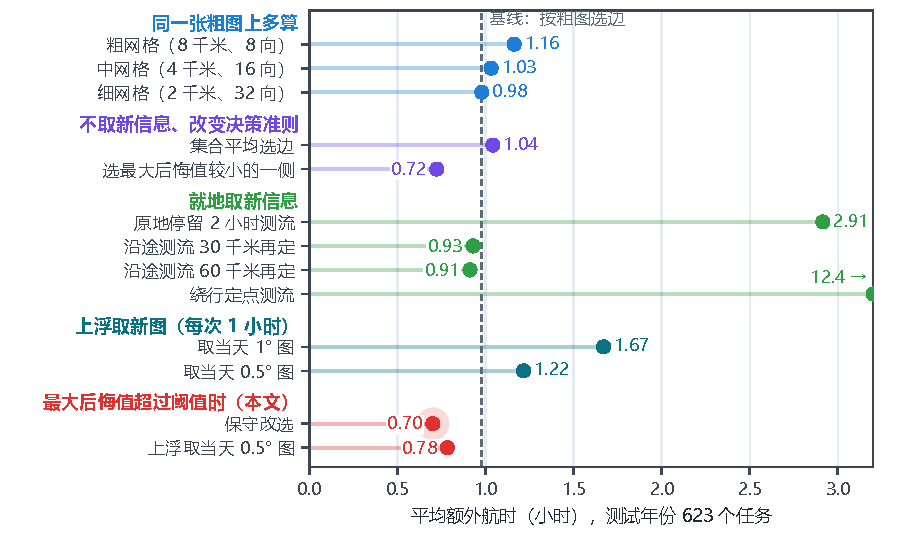
\includegraphics[width=0.88\linewidth]{fig_route_main}
\caption{黑潮测试年份623个任务上各类行动的平均额外航时（虚线为基线0.98小时，数值标在点旁）。由上至下依次为：同一张粗图上多算、不取新信息而改变选边准则、就地测流、总是上浮取图、最大后悔值超过阈值时的两种回应。加算与就地测流均未显著改善，超阈值时保守改选显著降低了额外航时。}
\label{fig:main}
\end{figure}

就地测流视野有限，多数情况下得不偿失（图\ref{fig:main}）。原地停留测流花2小时只测到起点一处；绕行定点测流平均要先花15.4小时赶到测点；沿途测流30千米很少改变判断（只有3.4\%的任务换边），测完60千米再换边又已走过半程。只有在额外航时很大的阿古拉斯回流区，沿途测流30千米才显著降低了额外航时，但仍不如上浮取图。

不能观测时，改选最大后悔值较小的一侧同样能降低额外航时。黑潮主设置中，超阈值时保守改选使平均额外航时从0.98小时降至0.70小时（配对差$-0.28$小时，95\%置信区间$[-0.51, -0.07]$）。它改选的41个任务中，23个改对、平均各省10.1小时，18个改错、平均各多花3.3小时：被避开的一侧往往有很大的下行风险，改对的收益远大于改错的代价。

\subsection{适用范围}
\label{sec:scope}
前两项发现在四种主要设置中都成立（第\ref{sec:compute}、\ref{sec:rank}节），回应的收益则取决于粗图误差的大小与结构（表\ref{tab:scope}）。粗图越可信，检验越少干预：航行器直接携带当天0.5°图时，基线的平均额外航时只有0.17小时，两种超阈值回应几乎不改变选边；航速降至0.75米/秒时，选错的代价增大，超阈值时上浮取图把额外航时从2.43小时降至1.32小时。用历史相似日的小尺度差代替标定的误差模型构造合理集合时，超阈值时保守改选（0.95小时）与基线（0.99小时）无显著差异，说明合理集合必须由真实的误差结构标定。

\begin{table}[tb]
\centering
\caption{各设置下的测试年份结果（额外航时单位：小时；上浮指取当天0.5°图）。}
\label{tab:scope}
\small
\begin{tabular}{@{}p{0.19\linewidth}>{\centering\arraybackslash}p{0.088\linewidth}>{\centering\arraybackslash}p{0.088\linewidth}>{\centering\arraybackslash}p{0.088\linewidth}>{\centering\arraybackslash}p{0.088\linewidth}>{\centering\arraybackslash}p{0.088\linewidth}>{\centering\arraybackslash}p{0.088\linewidth}>{\centering\arraybackslash}p{0.088\linewidth}@{}}
\toprule
设置 & 测试任务 & 存在合理反例 & 基线选错率 & 基线额外航时 & 超阈值时保守改选 & 超阈值时上浮取图 & 最大后悔值前20\%所占额外航时 \\
\midrule
黑潮主设置 & 623 & 99.7\% & 19.7\% & 0.98 & 0.70 & 0.78 & 67\% \\
粗图换成当天0.5°图 & 349 & 64.5\% & 8.0\% & 0.17 & 0.17 & 0.16 & 60\% \\
航速降至0.75米/秒 & 347 & 99.1\% & 18.4\% & 2.43 & 1.80 & 1.32 & 74\% \\
消融：合理集合改用相似日差值 & 349 & 99.4\% & 19.5\% & 0.99 & 0.95 & 0.77 & 64\% \\
湾流 & 643 & 98.8\% & 19.4\% & 3.56 & 4.00 & 1.31 & 71\% \\
阿古拉斯回流区 & 618 & 99.2\% & 27.7\% & 6.87 & 6.49 & 2.20 & 53\% \\
改带卫星测高地转流图 & 648 & 81.0\% & 19.6\% & 0.79 & 0.71 & 0.64 & 67\% \\
\bottomrule
\end{tabular}

\end{table}

不观测时的保守改选只适用于两侧最坏情形差别分明的海区。湾流与阿古拉斯回流区分别有8.7\%与16.2\%的任务在真实海流中有一侧无法通行（黑潮为1.0\%）；这类任务的合理集合中既有堵死左侧、也有堵死右侧的流场，两侧最大后悔值都接近上限，选较小的一侧近于随机，因此超阈值时保守改选在两海区均无显著收益。若只在两侧最大后悔值之差超过数值误差容限时才改选，这种近于随机的改选即可避免（湾流3.45小时，阿古拉斯回流区6.72小时，均与基线无显著差异）；在这两个海区，被标记的任务应交给上浮取图。

改带真实卫星测高地转流图时，加算无效与最大后悔值排序两项发现仍然成立（选错率从19.9\%变为19.6\%；前20\%的任务占67\%的额外航时），但各种回应均未显著降低额外航时，存在合理反例的任务也降至81.0\%。即使换成当天的测高图，选错率仍为18.5\%，而当天0.5°模式图只有8.6\%，说明测高图与再分析场之间的差异主要是两种产品的系统差，不随时效消失。

本研究仍有局限：单次任务中的海流视为定常；真实海流取自再分析场，平滑了亚中尺度过程；只考虑单个禁航区的左右选边；并假设选定一侧后航行器按真实海流以最优轨迹航行。

\section{原创创新点拆解}
\label{sec:innovation}

本研究从课程议题出发，经历了提出问题、实证否定与问题聚焦三个阶段。课上讲授的“海洋大数据的计算引擎”使作者联想到：航行器端侧的算力与能量有限，计算、测量与运动之间必须权衡。作者最初在东海赤潮巡测场景下研究机载计算与观测的时间分配，发现多算只会抬高规划器的自我估值（图\ref{fig:curse}），而时间分配本身的改进空间也很小：出发前模拟选出的分配策略平均遗憾为0.265，事后为每个任务挑选最优策略也只能降到0.243，远小于下水位置（约0.13）与信息新鲜度（约0.03）的影响。作者据此指出该方法增益小、新意不足，并把问题聚焦到选错一侧就要多花数小时的绕障选边：既然多算无法区分不同的真实海洋，能否直接检验是否存在与粗图相容、却使另一侧更快的合理反例？这一追问形成了本文的研究问题与表\ref{tab:innovation}所列的四个创新点。

\begin{table}[tb]
\centering
\caption{原创创新点、已有做法、实验证据与局限。}
\label{tab:innovation}
\footnotesize
\begin{tabular}{@{}p{0.13\linewidth}p{0.20\linewidth}p{0.22\linewidth}p{0.19\linewidth}p{0.14\linewidth}@{}}
\toprule
创新点 & 已有做法及其不足 & 本文做法 & 证据 & 局限 \\
\midrule
1. 区分数值歧义与环境歧义 & 加密网格或增加推演，把求解误差与信息缺失混为一谈。 & 以“能否找到合理反例”判定歧义的性质：数值歧义交给计算，环境歧义交给观测。 & 图\ref{fig:ambiguity}：加算64倍选错率仅从21.7\%降至19.7\%，换当天0.5°图降至10.4\%。 & 只在单个禁航区的左右选边上验证。 \\
\addlinespace
2. 用海洋大数据标定合理集合 & 凭经验设定不确定集，或借用历史相似日的差值。 & 用多年误差标定逐点误差、76千米相关长度的无散模态与覆盖90\%以上真实情况的半径。 & 图\ref{fig:data}、表\ref{tab:scope}：测试年份覆盖94\%；改用相似日差值后检验失效。 & 依赖历史统计，对台风等极端过程适应有限。 \\
\addlinespace
3. 最大后悔值的梯度搜索 & 随机抽样需上千个成员；改变选边的成员比例不计代价大小。 & 沿最快航线按包络定理求导，每次迭代2次求解，直接搜索最大后悔值。 & 图\ref{fig:risk}、\ref{fig:budget}：约71次求解达到2048次求解的效果；前20\%任务占53\%--71\%额外航时。 & 流场变化大时最快航线可能改变，一阶近似有误差。 \\
\addlinespace
4. 粗图不可信时先取新信息 & 不论风险一律观测或一律不观测。 & 最大后悔值超过阈值才付出观测代价；不能观测时改选最大后悔值较小的一侧。 & 图\ref{fig:main}、表\ref{tab:scope}：湾流与阿古拉斯回流区的额外航时降至1.31与2.20小时。 & 不观测时的保守改选只在黑潮主设置显著。 \\
\bottomrule
\end{tabular}
\end{table}

人机分工见附录B：研究问题与方向由作者提出并把关；Claude（Anthropic）完成文献检索、代码、实验与作图，并按作者要求重构撰写了本文终稿；此前各稿由Gemini（Google）根据Claude整理的事实清单撰写。

\section{结论}
\label{sec:conclusion}

本文研究了自主水下航行器携带陈旧粗图绕障选边时，应当继续计算还是获取新信息的问题，提出了合理反例检验：用多年再分析数据标定与粗图相容的合理流场集合，以包络定理梯度搜索使另一侧更快的合理反例，并以最大后悔值判定粗图对当前决定是否可信。四种设置共2532个测试任务的实验表明，计算量增加64倍几乎不改变选错率，而几乎每个决定都存在合理反例；最大后悔值能把额外航时集中到少数任务上；在粗图误差大的海区，判定不可信后上浮取图使平均额外航时降低六成以上。不观测的保守改选只在两侧最坏情形差别分明的海区有效，改带真实卫星测高图时各种应对的收益也不再显著。

更一般地，海洋大数据的计算正在向航行器端侧延伸，但端侧计算只能把已有的信息算准，补不回海流图中缺失的信息。合理反例检验为端侧智能体在计算与观测之间的取舍提供了可计算的判据，可为长航程航行器的自主决策提供支撑。未来工作将把该方法推广到时变流场与多障碍物的航路选择，并开展实艇海试。


% ---------- 参考文献 ----------
\phantomsection
\bibliographystyle{gbt7714-numerical}
\bibliography{refs}

% ---------- 附录 ----------
\appendix
{\sloppy\section*{附录}

\subsection*{附录 A：代码与数据开源说明}
本研究的全部源代码、数据处理脚本、实验配置、统计汇总程序以及论文图表生成脚本均已开源于代码仓库：\url{https://github.com/frankxucd0826-source/auv-compute-or-observe}。

\begin{enumerate}
    \item \textbf{数据集来源：}主实验海流数据取自HYCOM全球海洋再分析公开服务（产品GLBy0.08，实验93.0，10米水深水平流速，黑潮主设置区域23°--31°N、121°--129°E，2019--2024年；重复实验区为湾流33°--41°N、75°--67°W与阿古拉斯回流区35°--43°S、14°--22°E，产品与时间范围相同；黑潮区改带卫星测高地转流图检验所用的近实时融合测高地转流取自美国国家海洋和大气管理局海岸观测网数据服务）；附录B所述前期探索的叶绿素与海表温度数据取自同一数据服务的公开卫星产品。
    \item \textbf{主要程序结构：}核心软件包 \texttt{src/oceanroute/} 包含网格最短路与包络定理梯度求解器（\texttt{solver.py}）、海流快照与粗图（\texttt{fields.py}，海区与粗图来源分别由环境变量 \texttt{OCEANROUTE\_REGION}、\texttt{OCEANROUTE\_MAP} 选择）、粗图误差的多年数据标定与无散误差模态（\texttt{errormodel.py}）以及任务生成、合理反例检验与测量更新（\texttt{mission.py}）；数据下载、批量评估、统计汇总、集合成员对照与各海区实验分别由 \texttt{scripts/download\_hycom.py} 与 \texttt{experiments/route\_*.py} 完成，正文插图由 \texttt{paper/figures/route*\_*.py} 生成，图\ref{fig:overview}中心的三维示意由 \texttt{paper/figures/blender/render\_route.py} 用开源软件Blender渲染，海面与流场纹理取自示例任务的真实数据；逐条复现命令与前期探索的脚本见仓库根目录的 \texttt{README}。
\end{enumerate}

\subsection*{附录 B：研究过程与人工智能工具使用说明}
\textbf{研究过程。}本研究从课程议题出发，经历了提出问题、自我否定与问题聚焦三个阶段。课上讲授的“海洋大数据的计算引擎”使作者联想到：航行器端侧的算力与能量有限，计算、测量与运动之间必须权衡。作者最初在东海赤潮巡测场景下研究机载计算与观测的时间分配，结果显示时间分配本身的改进空间很小，而出发前预演又是机器人领域的常用策略；作者据此判断该方向增益小、新意不足，并追问：多算之所以帮不上忙，是否因为粗图本身容许多种真实海洋？若是，能否直接检验是否存在与粗图相容、却使另一侧更快的流场？这一追问把问题聚焦到选错一侧就要多花数小时的绕障选边，形成了本文的研究问题与第\ref{sec:diff}节所列的三个创新点。

\textbf{人工智能工具的使用。}本研究与论文撰写中人工智能工具的使用情况如下：
\begin{enumerate}
    \item \textbf{作者：}提出了机载计算与现场观测如何权衡的初始问题；对第一版结果提出用真实卫星数据检验、补充对照与消融、按学术论文格式写作等要求；在前期研究结果出来后指出其提升小、新意不足，并提出“粗分辨率海流图下两条航路的合理反例”这一新问题，决定转向本文研究；在重复实验完成后，要求以各设置下都成立的结论为主线改写全文，理顺逻辑、不用自造术语并压缩篇幅；随后指出图文排版、创新点突出程度与段落逻辑的不足，指出引言不应以前期探索中增益不大的内部结果为依据，要求重画全部插图并重写全文；又指出语言绕、缺少“已有方法为何失效、因此怎样做”的逻辑链、摘要看不出用什么方法解决了什么问题，要求按摘要八步法与逐段排除常规做法的写法重写，并把原创创新点拆解从文末移到更合适的位置；对全文负责。
    \item \textbf{Claude（Anthropic）：}在作者授权下完成文献检索与核对、数据下载与全部代码、实验与统计、论文插图，整理写作提纲与由实验程序生成的事实清单，逐项核对正文中的数字与引用，并按作者要求重构撰写了论文终稿。
    \item \textbf{Gemini（Google）：}根据Claude整理的提纲、术语表与事实清单撰写了论文此前的各稿，由Claude核对与修改。
    \item \textbf{可追溯性记录：}作者与人工智能工具的对话记录、与Gemini的每轮写作往来以及研究笔记均保存在上述代码仓库中（涉及作者其他未发表工作的内容已隐去）。
\end{enumerate}
\par}

\end{document}
